\section*{Beispiel}

\begin{frame}{Eingabe-Graph}
    \begin{figure}[h]
        \centering
        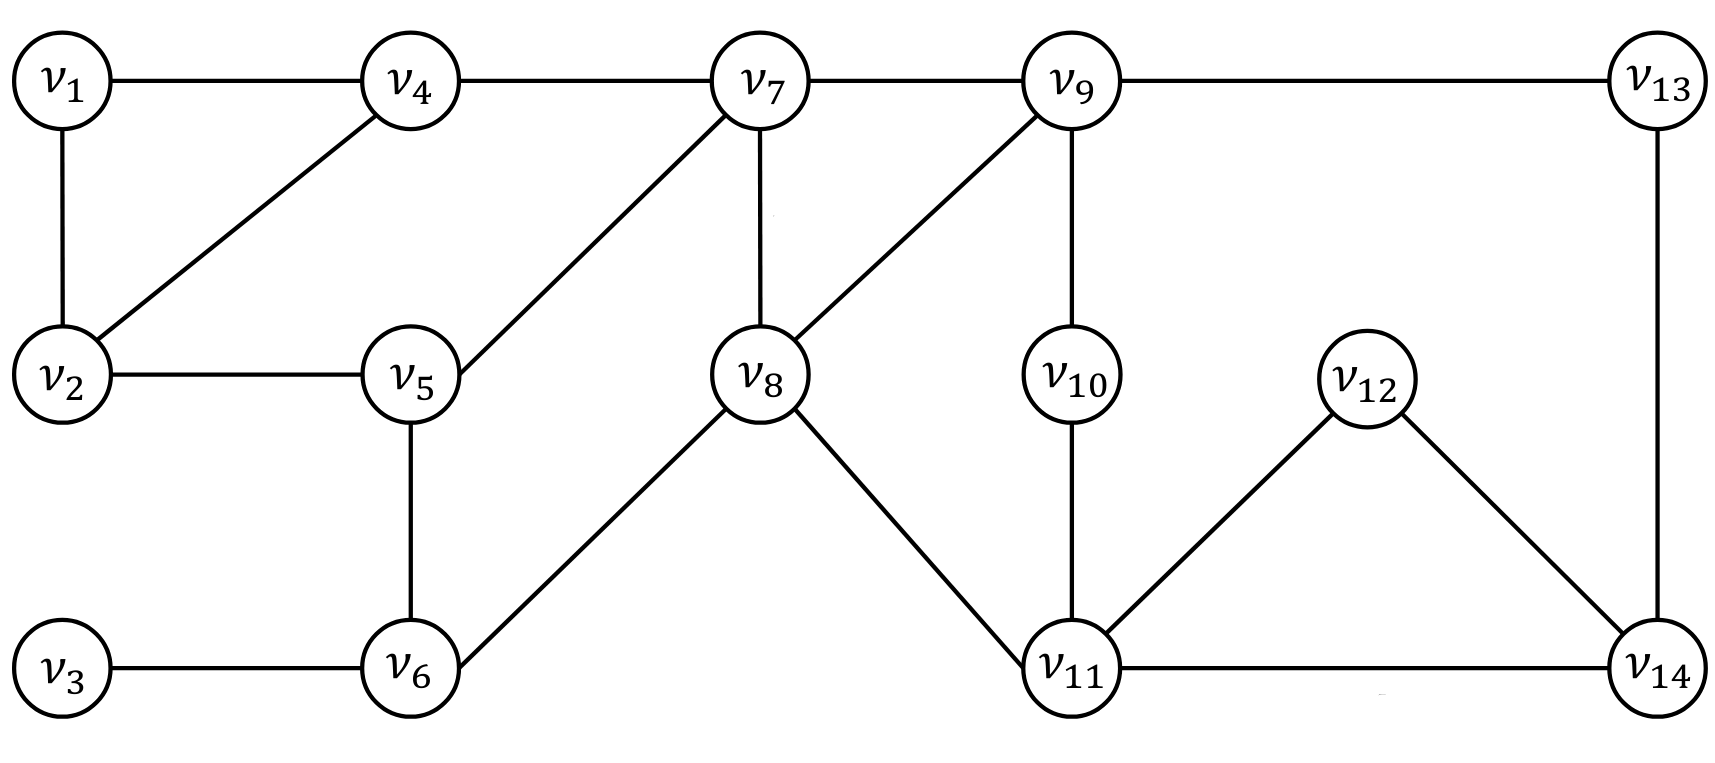
\includegraphics[width=0.9\textwidth]{imglib/Example-Graph-Initial}\\
        \label{fig:example-graph-initial}
    \end{figure}
\end{frame}

\begin{frame}{Visualisierte Ausgabe für h = 1}
    \begin{figure}[h]
        \centering
        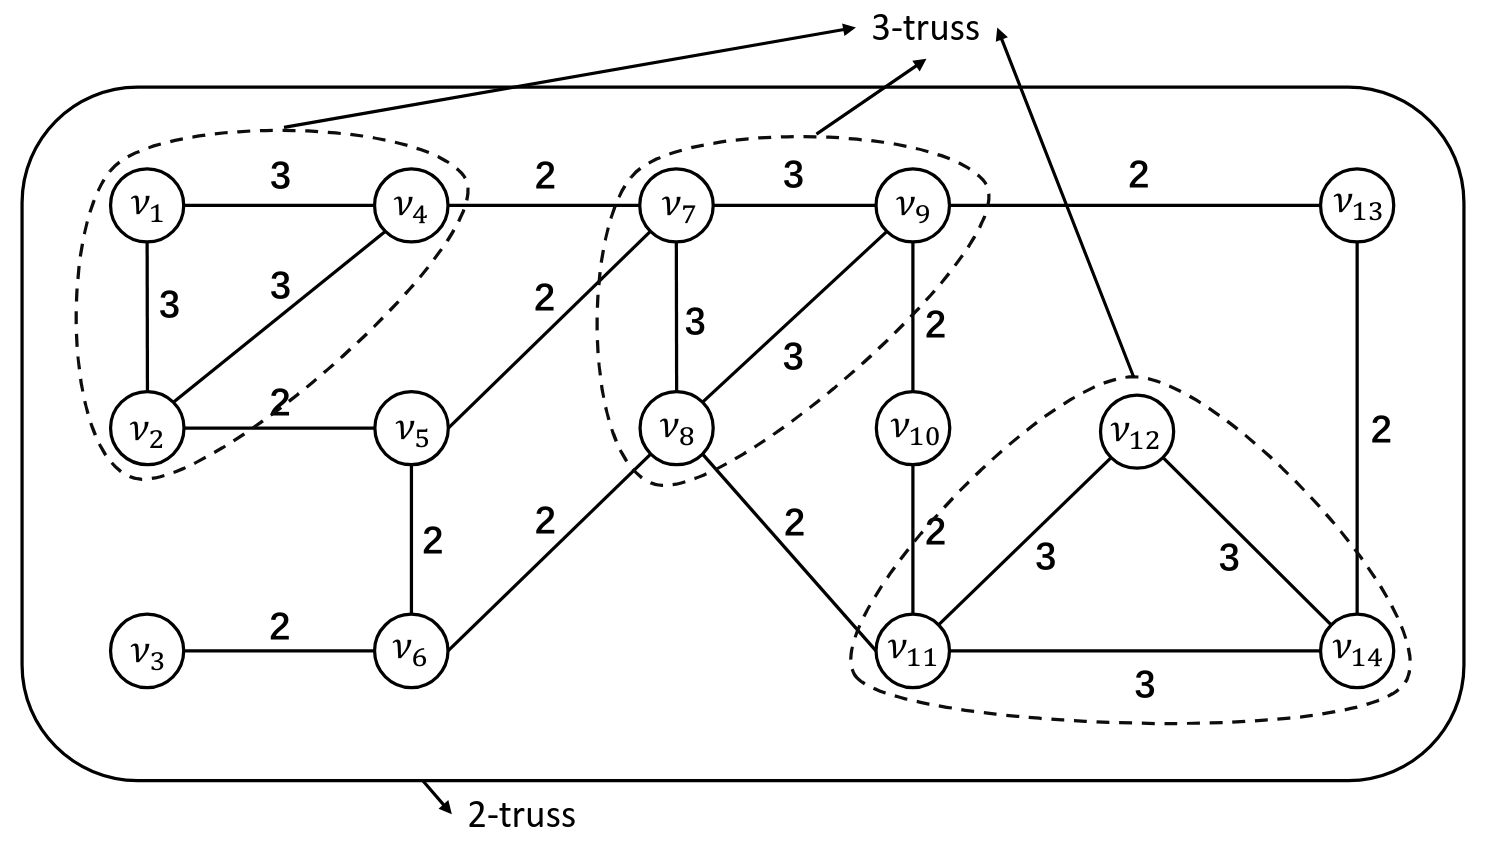
\includegraphics[width=0.7\textwidth]{imglib/Example-Graph-Solution-1}\\
        \label{fig:example-graph-solution-1}
    \end{figure}
\end{frame}

\begin{frame}{Visualisierte Ausgabe für h = 2}
    \begin{figure}[h]
        \centering
        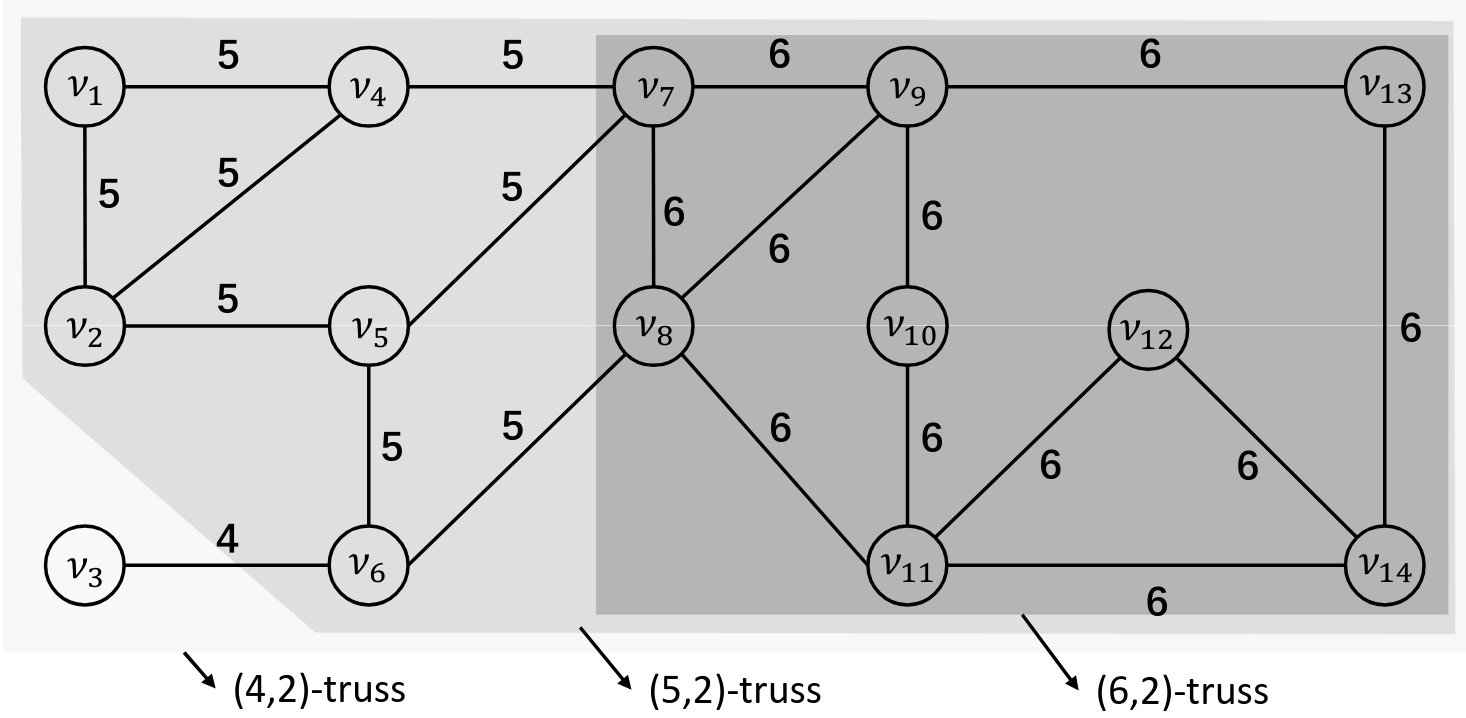
\includegraphics[width=0.7\textwidth]{imglib/Example-Graph-Solution-2}\\
        \label{fig:example-graph-solution-2}
    \end{figure}
\end{frame}